\documentclass{article}

\usepackage{graphicx}
\usepackage{tikz}
\usepackage{tikzsymbols}
\usetikzlibrary{calc,patterns,shapes.geometric}
\pagestyle{empty}
\usepackage[margin=0pt]{geometry}
\geometry{papersize={14in,12in}}

\def\centerarc[#1](#2)(#3:#4:#5){\draw[#1] ($(#2)+({#5*cos(#3)},{#5*sin(#3)})$) arc (#3:#4:#5);}

\begin{document}
	\begin{figure}
		\centering
		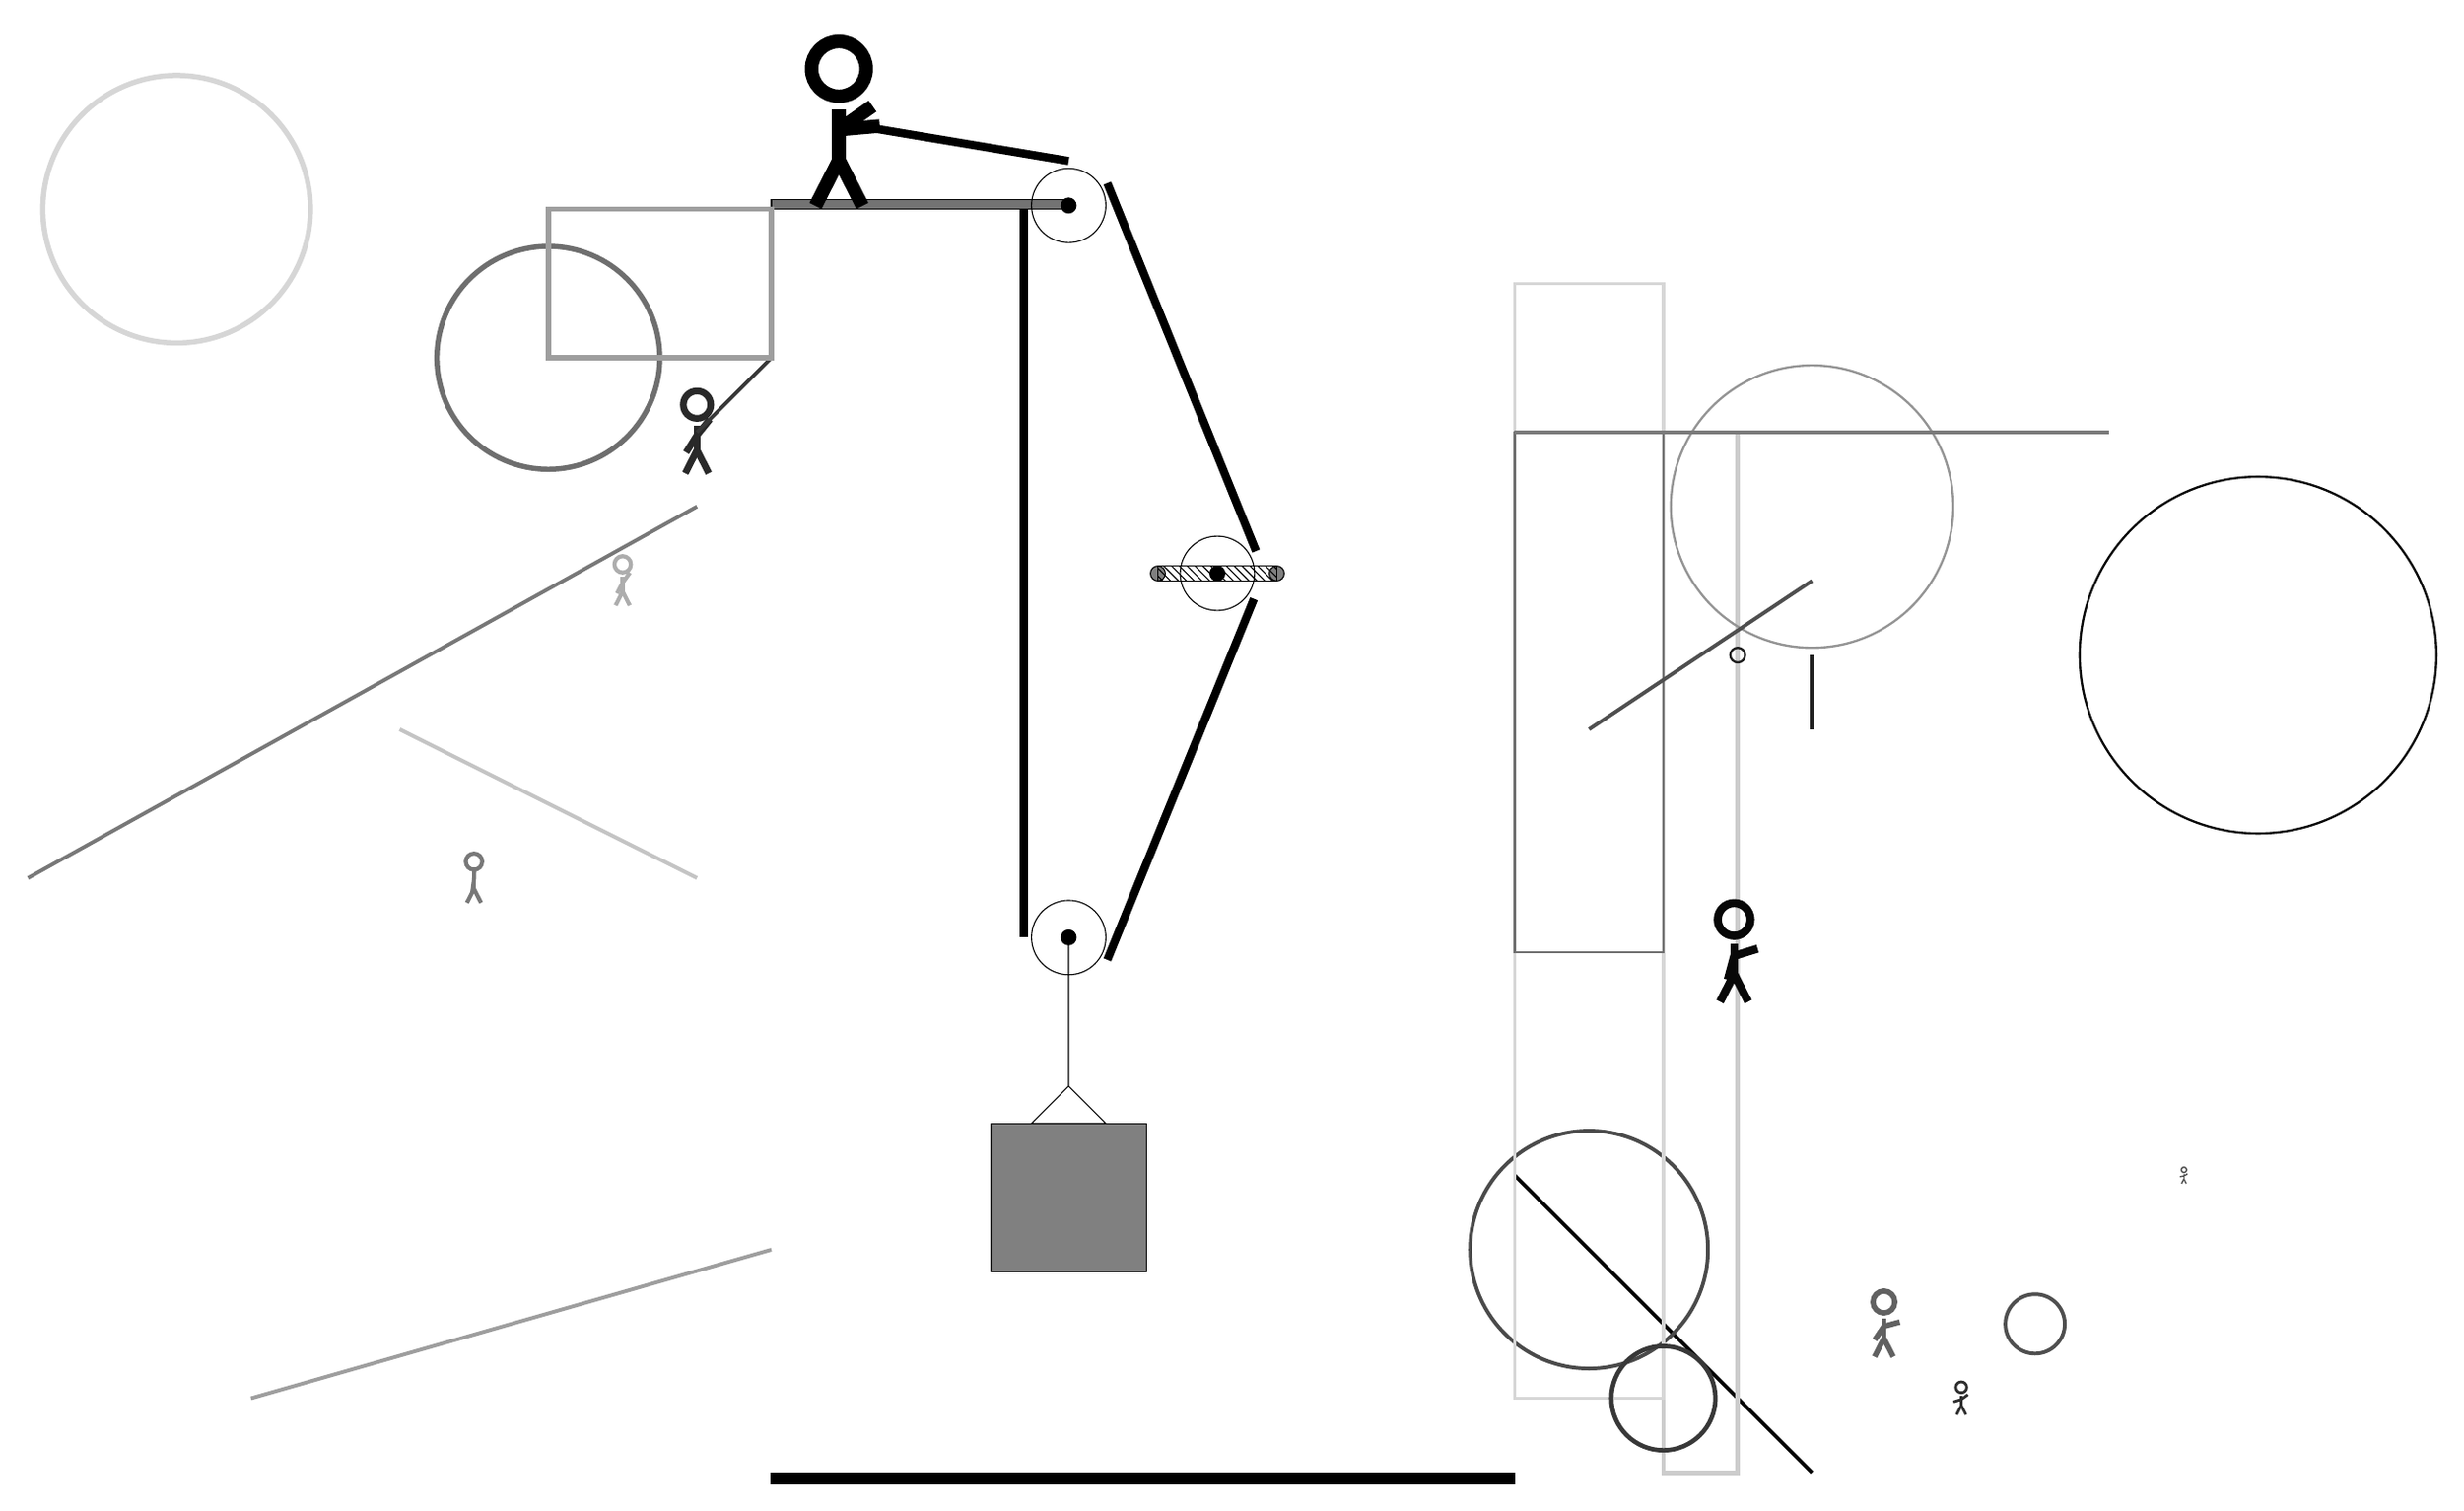
\begin{tikzpicture}
			%%%%% START %%%%%
			
			\draw[fill=black!55] (-2, 14) rectangle (2, 14.125);
			
			\draw (2, 4.2) circle (0.5);
			\draw[fill=black] (2, 4.2) circle (0.1);
			
			\draw (2, 14.05) circle (0.5);
			\draw[fill=black] (2, 14.05) circle (0.1);
			
			\draw[fill=white](4, 9.1) circle (0.5);
			\draw[fill=black] (4, 9.1) circle (0.1);
			\draw[fill=black!50] (3.2, 9.1) circle (0.1);
			\draw[fill=black!50] (4.8, 9.1) circle (0.1);
			\draw[pattern=north west lines, pattern color=black] (3.2, 9.2) rectangle (4.8, 9.0);
			
			\draw (2, 4.2) -- (2, 2.2) -- (1.5, 1.7) -- (2.5, 1.7) -- (2, 2.2);
			\draw[fill=black!50] (0.95, 1.7) rectangle (3.05, -0.3);
			
			\draw[line width=1.1mm] (1.4, 14) -- (1.4, 4.2);
			\centerarc[line width=1.1mm](2, 4.2)(180:330:0.6);
			\draw[line width=1.1mm](2.5196, 3.9) -- (4.4915, 8.7558);
			\centerarc[line width=1.1mm](4, 9.1)(390:325:0.6);
			\draw[line width=1.1mm](4.5196, 9.4) -- (2.5196, 14.35);
			\centerarc[line width=1.1mm](2, 14.05)(30:90:0.6);
			\draw[line width=1.1mm](2, 14.65) -- (-1, 15.15);
			
			\node at (-1, 15.15) {\Strichmaxerl[10][-175][35]};
			
			\node[line width=0.2mm, color=black!32] at (-4, 9) {\Strichmaxerl[3][63][54]};
			
			\draw[line width=0.5mm, color=black!23](-3, 5) -- (-7, 7);
			\node[line width=0.5mm, color=black!69] at (17, 1) {\Strichmaxerl[1][11][30]};
			\node[line width=0.4mm, color=black!84] at (-3, 11) {\Strichmaxerl[5][58][51]};
			
			\draw[line width=0.5mm, color=black!99](12, -3) -- (8, 1);
			\draw [line width=0.5mm, color=black!71](9, 0) circle (1.6);
			
			\draw[line width=0.6mm, color=black!20] (10, -3) rectangle (11, 11);
			\draw [line width=0.3mm, color=black!42](12, 10) circle (1.9);
			\draw[line width=0.5mm, color=black!53](-3, 10) -- (-12, 5);
			\node[line width=0.7mm, color=black!97] at (11, 4) {\Strichmaxerl[6][75][17]};
			
			\draw[line width=0.5mm, color=black!78](-3, 11) -- (-2, 12);
			
			\draw[line width=0.4mm, color=black!16] (10, 13) rectangle (8, -2);
			\draw[line width=0.3mm, color=black!57] (8, 4) rectangle (10, 11);
			
			\draw [line width=0.5mm, color=black!69](15, -1) circle (0.4);
			\node[line width=0.3mm, color=black!82] at (14, -2) {\Strichmaxerl[2][17][36]};
			\draw[line width=0.5mm, color=black!69](9, 7) -- (12, 9);
			
			\draw[line width=0.5mm, color=black!87](12, 7) -- (12, 8);
			
			\draw [line width=0.7mm, color=black!16](-10, 14) circle (1.8);
			\draw [line width=0.6mm, color=black!78](10, -2) circle (0.7);
			\draw [line width=0.7mm, color=black!57](-5, 12) circle (1.5);
			\draw [line width=0.3mm, color=black!89](11, 8) circle (0.1);
			\draw[line width=0.5mm, color=black!52](8, 11) -- (16, 11);
			\draw[line width=0.7mm, color=black!38] (-2, 12) rectangle (-5, 14);
			\node[line width=0.7mm, color=black!53] at (-6, 5) {\Strichmaxerl[3][82][88]};
			\node[line width=0.5mm, color=black!62] at (13, -1) {\Strichmaxerl[4][56][15]};
			
			\draw [line width=0.3mm, color=black!96](18, 8) circle (2.4);
			
			\draw[line width=0.5mm, color=black!38](-2, 0) -- (-9, -2);
			
			\draw[fill=black] (-2, -3) rectangle (8, -3.15);
			
			%%%%% END %%%%%
		\end{tikzpicture}
	\end{figure}	
\end{document}